\documentclass{beamer}
\usetheme{Boadilla}

\usepackage{graphicx}
\usepackage{subcaption}
\usepackage{csvsimple}

% Change size of footnotes
\renewcommand{\footnotesize}{\fontsize{5pt}{5pt}\selectfont}
\title{Analysis of gene regulatory properties underlying pleiotropy between complex traits}
\subtitle{Meeting GOLD 2022}
\author{Aitor Gonz\'alez}
\institute{Aix Marseille Univ, INSERM, TAGC}
\date{Oct. 19, 2022}

% Add section slide
\AtBeginSection[]
{
\begin{frame}
\frametitle{Table of Contents}
\tableofcontents[currentsection]
\end{frame}
}

\begin{document}

%%%%%%%%%%%%%%%%%%%%%%%%%%%%%%%%%%%%%%%%%%%%%%%%%%%%%%%%%%%%%%%%%%%%%%%%%%%%%%%%
\begin{frame}

\titlepage

\end{frame}


\section{Introduction} %%%%%%%%%%%%%%%%%%%%%%%%%%%%%%%%%%%%%%%%%%%%%%%%%%%%%%%%%%%%%%

%%%%%%%%%%%%%%%%%%%%%%%%%%%%%%%%%%%%%%%%%%%%%%%%%%%%%%%%%%%%%%%%%%%%%%%%%%%%%%%%
\begin{frame}
\frametitle{Genome-wide association studies (GWAS)}

\begin{itemize}
\item Genetic alleles with higher frequency in individuals with a given disease
\item A very active field with many studies
\item Many genetic variants are involved in several phenotypes
\end{itemize}
%
\vfill
%
Questions:
%
\begin{itemize}
\item Correlation between variants. Which is the causal variant?
\item Which cell type important for disease?
\item Over 90\% GWAS variants are non-coding. What is their role?
\end{itemize}
%
\vfill
%
Questions partially addressed by looking at eQTLs in different tissues

\let\thefootnote\relax\footnotetext{Cano-Gamez et al. 2020. doi:10.3389/fgene.2020.00424}

\end{frame}

%%%%%%%%%%%%%%%%%%%%%%%%%%%%%%%%%%%%%%%%%%%%%%%%%%%%%%%%%%%%%%%%%%%%%%%%%%%%%%%%
\begin{frame}
\frametitle{Expression quantitative trait loci (eQTL)}

\begin{columns}
\begin{column}{0.5\textwidth}
    \begin{center}
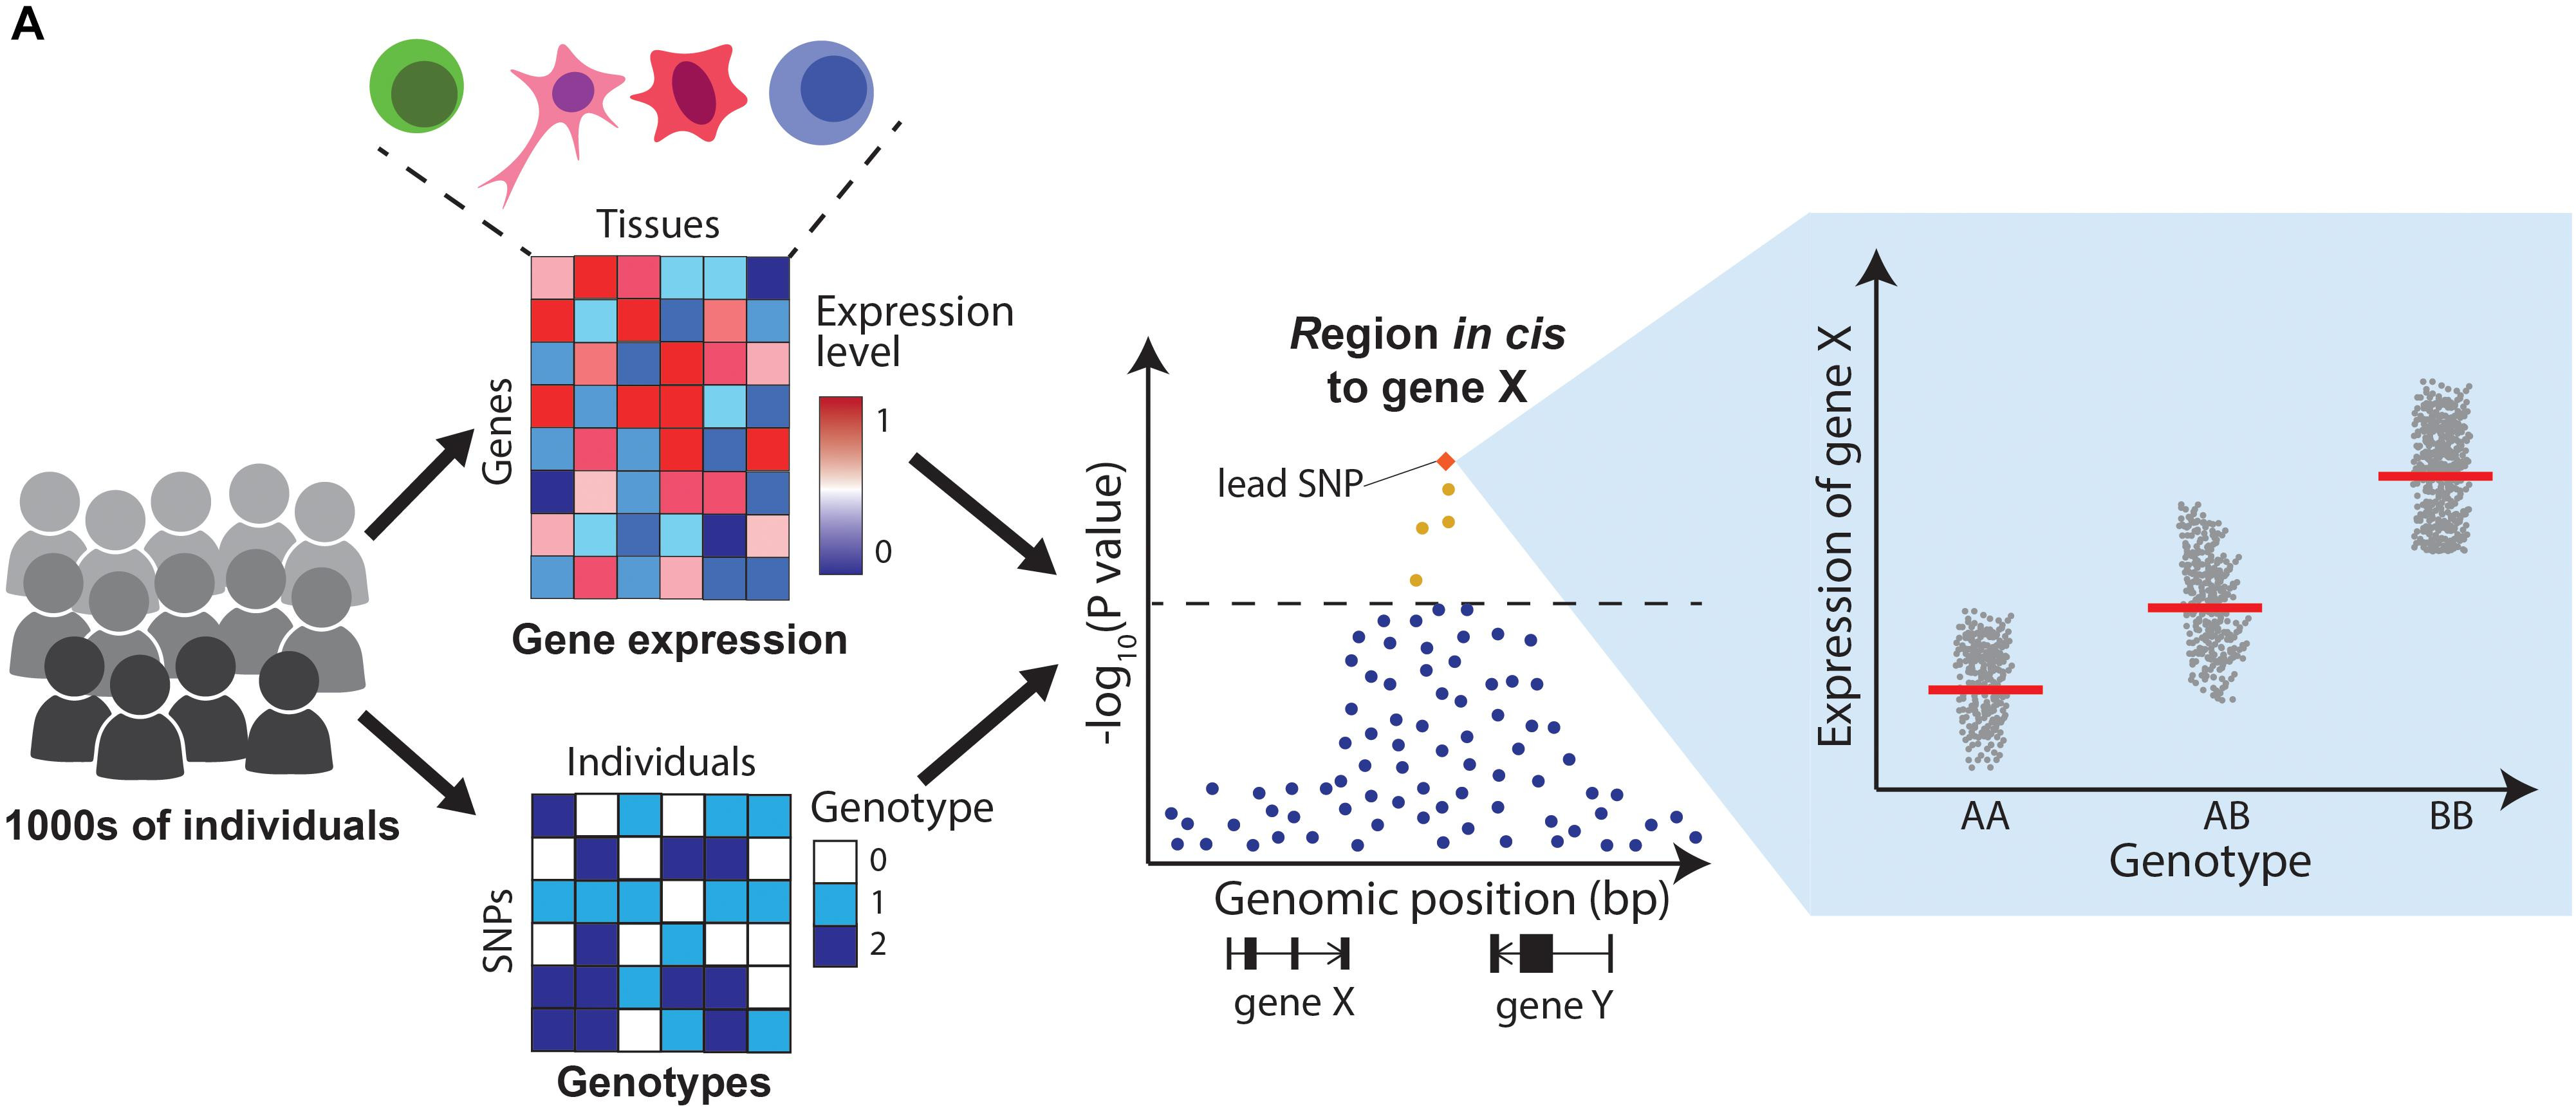
\includegraphics[width=\textwidth]{/home/gonzalez/Repositories/gwas2eqtl_pleiotropy/presentation_gold2022_paris/fig/doi_10.3389_fgene.2020.00424_fig4a.jpg}
     \end{center}
\end{column}
\begin{column}{0.5\textwidth}

\end{column}
\end{columns}

\let\thefootnote\relax\footnotetext{Cano-Gamez et al. 2020. doi:10.3389/fgene.2020.00424}
\end{frame}

%%%%%%%%%%%%%%%%%%%%%%%%%%%%%%%%%%%%%%%%%%%%%%%%%%%%%%%%%%%%%%%%%%%%%%%%%%%%%%%%
\begin{frame}
\frametitle{Annotation of GWAS variants with gene and tissue targets using colocalization analysis}

\begin{columns}
\begin{column}{0.5\textwidth}
    \begin{center}
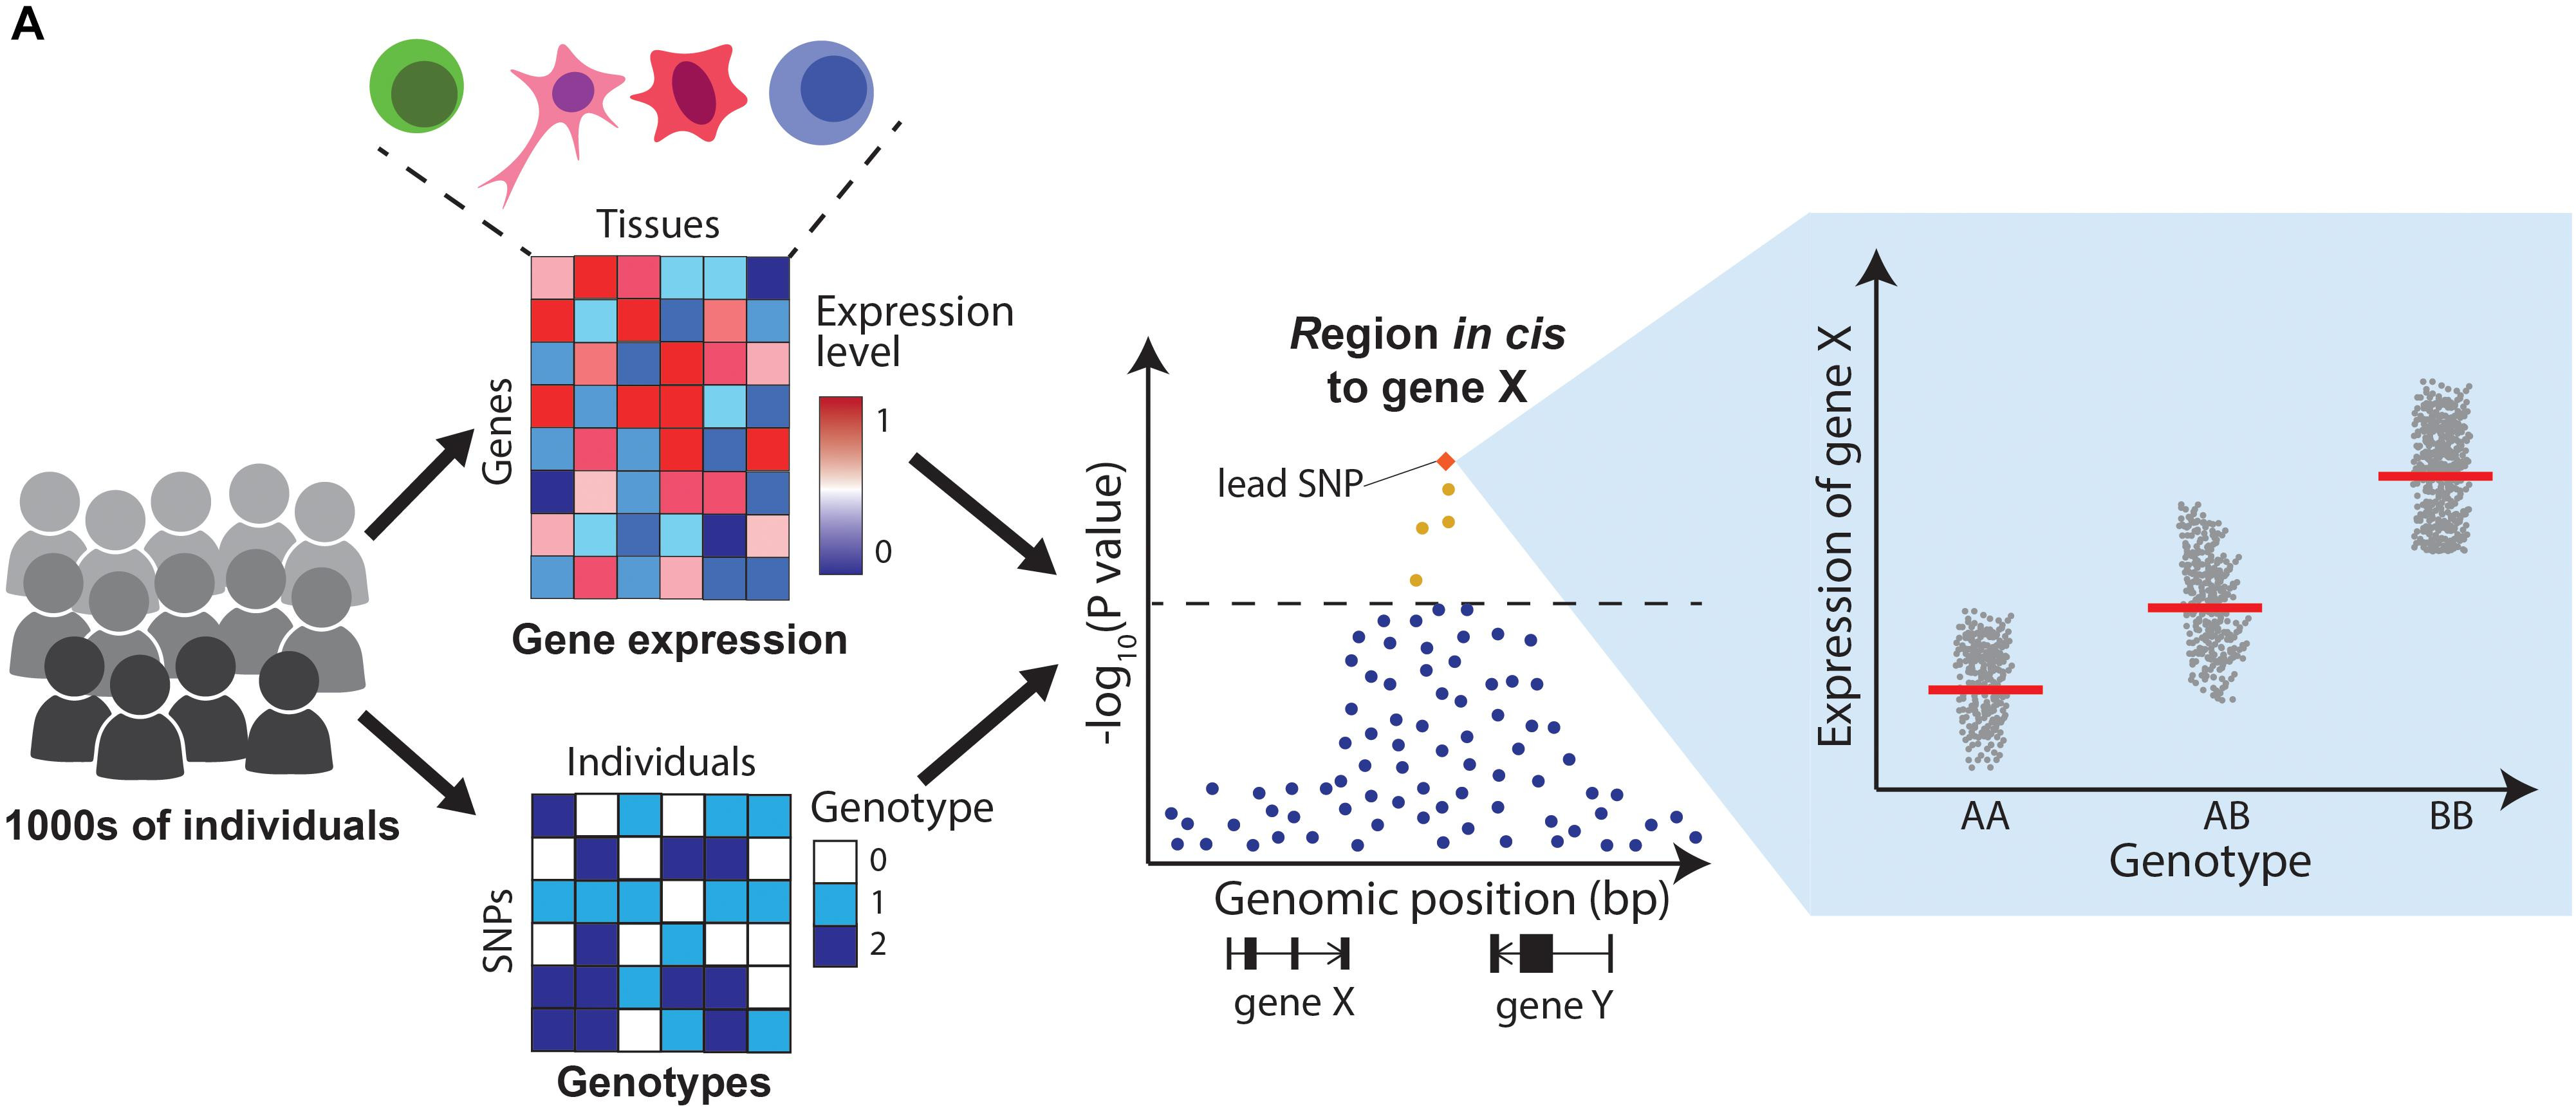
\includegraphics[width=\textwidth]{/home/gonzalez/Repositories/gwas2eqtl_pleiotropy/presentation_gold2022_paris/fig/doi_10.3389_fgene.2020.00424_fig4a.jpg}
     \end{center}
\end{column}
\begin{column}{0.5\textwidth}
    \begin{center}
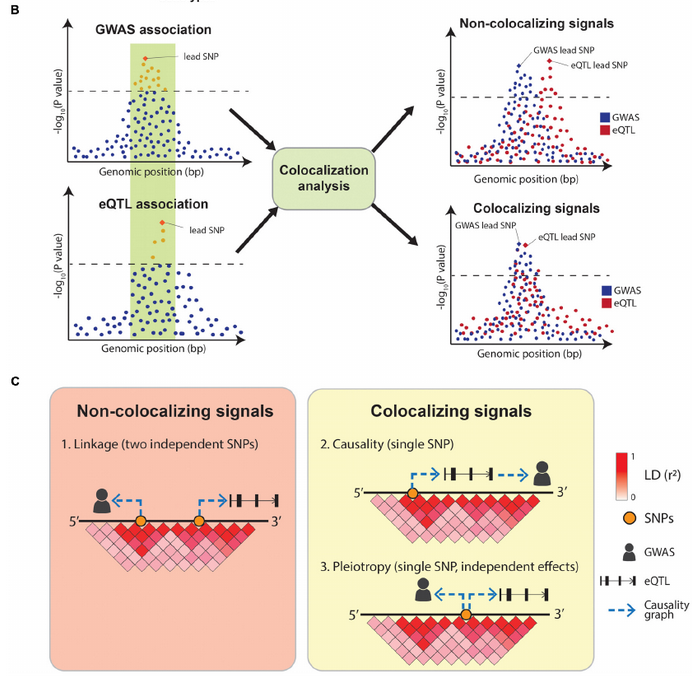
\includegraphics[width=\textwidth]{/home/gonzalez/Repositories/gwas2eqtl_pleiotropy/presentation_gold2022_paris/fig/doi_10.3389_fgene.2020.00424_fig4bc.png}
     \end{center}
\end{column}
\end{columns}

\let\thefootnote\relax\footnotetext{Cano-Gamez et al. 2020. doi:10.3389/fgene.2020.00424}
\end{frame}

%%%%%%%%%%%%%%%%%%%%%%%%%%%%%%%%%%%%%%%%%%%%%%%%%%%%%%%%%%%%%%%%%%%%%%%%%%%%%%%%
\begin{frame}
\frametitle{Objectives}

\begin{enumerate}
\item Large scale gene and tissue annotation of variants of complex traits using GWAS/eQTL colocalization analysis
\item To identify genetic variants leading to pleiotropy of complex traits
\item To characterize the gene regulatory mechanisms of trait pleiotropy
\end{enumerate}
\end{frame}

%%%%%%%%%%%%%%%%%%%%%%%%%%%%%%%%%%%%%%%%%%%%%%%%%%%%%%%%%%%%%%%%%%%%%%%%%%%%%%%%
\begin{frame}
\frametitle{Data and Algorithms}

\begin{columns}
\begin{column}{0.5\textwidth}
\begin{itemize}
\item IEA OpenGWAS database$^1$: 244,881e6 associations from 42e3 GWAS datasets
\item EBI eQTLs database$^2$: Processed gene expression and splicing QTLs from all public studies on human.
\item CRAN - Package coloc$^3$: Genetic colocalisation analysis of two phenotypes to look for shared common genetic causal variants
\end{itemize}
\end{column}
\begin{column}{0.5\textwidth}
\begin{center}
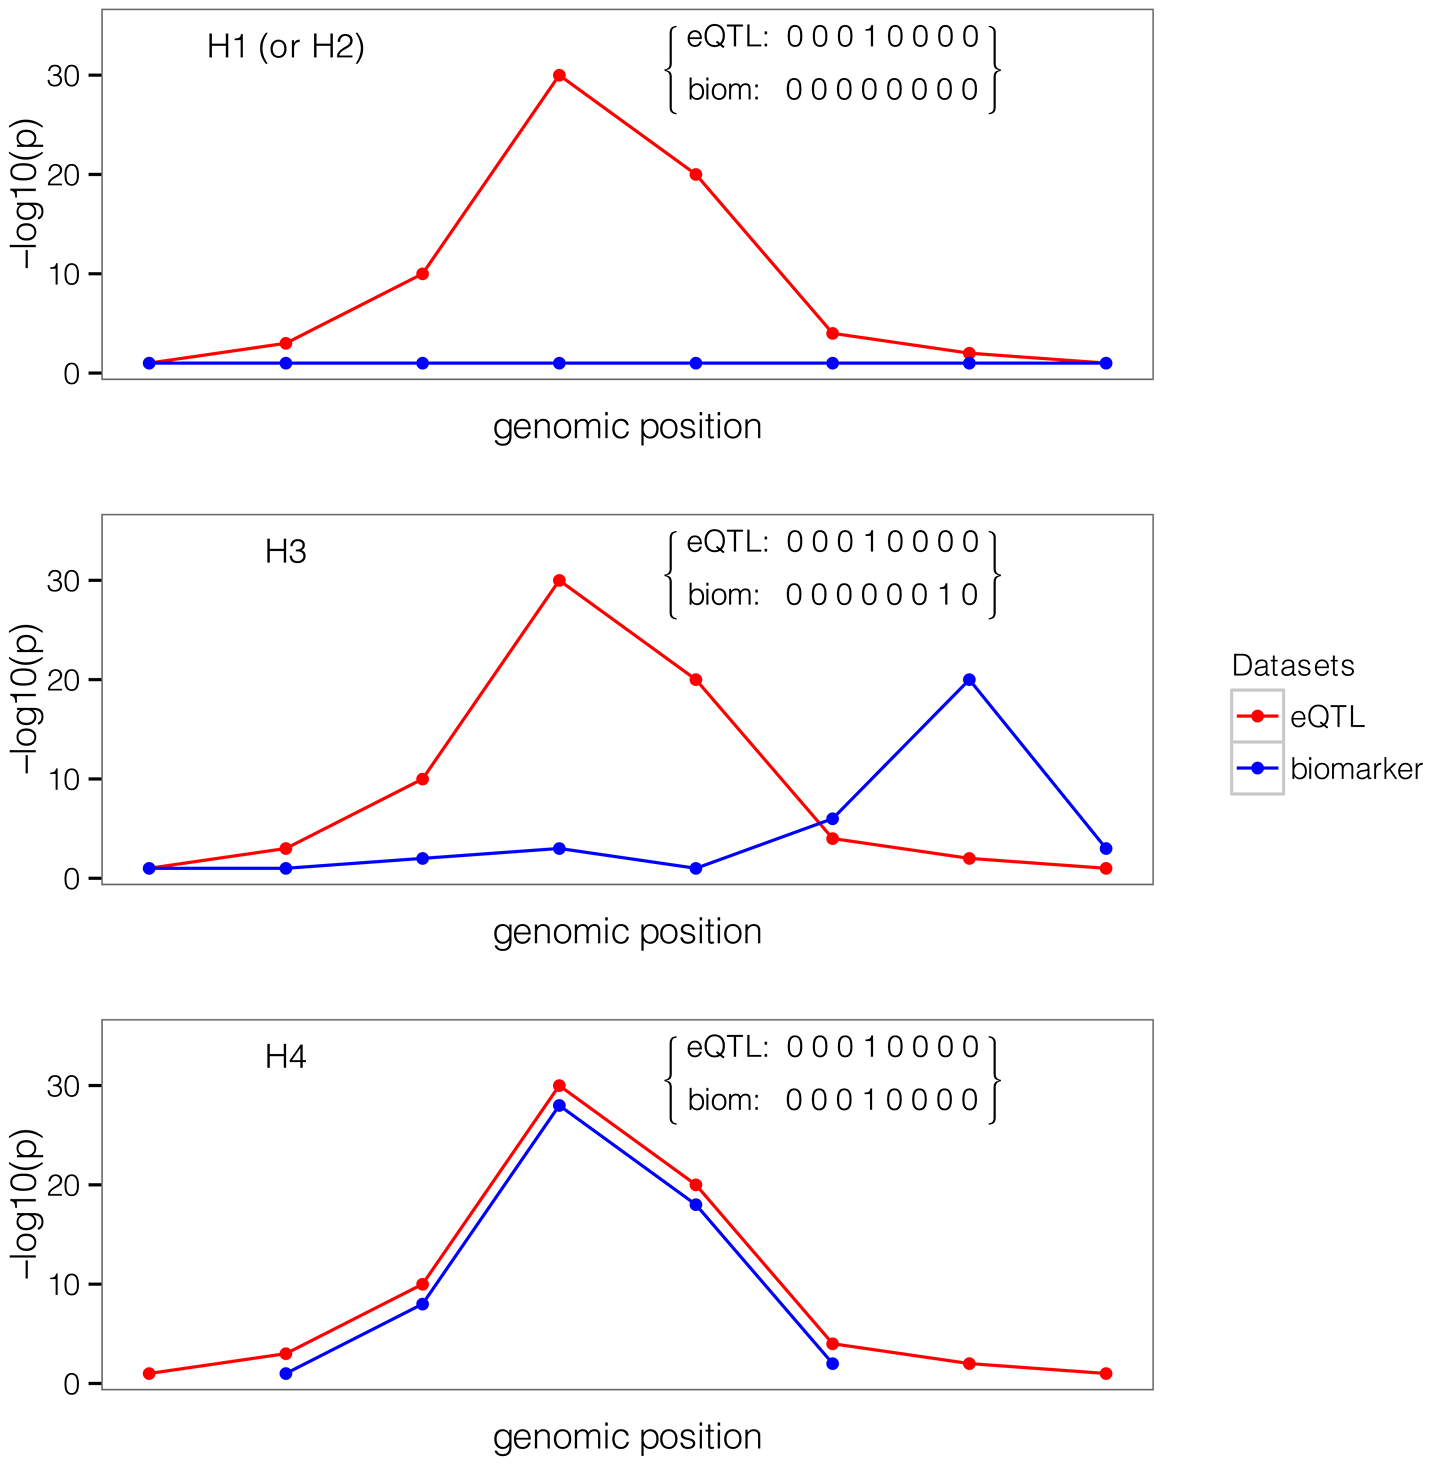
\includegraphics[width=\textwidth]{/home/gonzalez/Repositories/gwas2eqtl_pleiotropy/presentation_gold2022_paris/fig/pgen.1004383.g001.png}
\end{center}
\end{column}
\end{columns}

\let\thefootnote\relax\footnotetext{$^1$https://gwas.mrcieu.ac.uk}
\let\thefootnote\relax\footnotetext{$^2$https://www.ebi.ac.uk/eqtl}
\let\thefootnote\relax\footnotetext{$^3$https://cran.r-project.org/web/packages/coloc/index.html}
\end{frame}


\section{Results}

%%%%%%%%%%%%%%%%%%%%%%%%%%%%%%%%%%%%%%%%%%%%%%%%%%%%%%%%%%%%%%%%%%%%%%%%%%%%%%%%
\begin{frame}
\frametitle{Large scale GWAS/eQTL colocalization analysis}

\begin{itemize}
\item Colocalization analysis of 418 GWAS and 127 eQTL studies (53e3 pairs)
\item 143e3 shared causal variants with probability $\geq$ 0.8
\item Percentage of GWAS loci explained by eQTL: 0$\%$ - 77$\%$ (Average 33$\%$)
\end{itemize}

\begin{figure}[!]
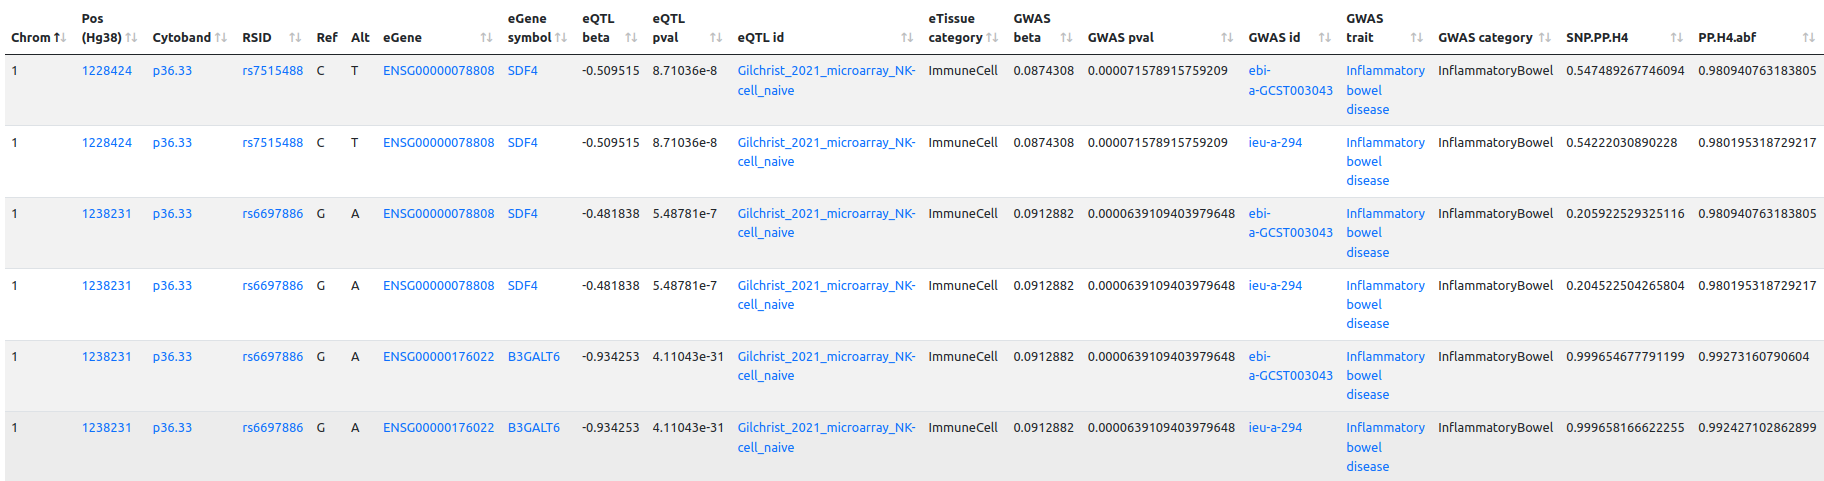
\includegraphics[width=\textwidth]{/home/gonzalez/Repositories/gwas2eqtl_pleiotropy/presentation_gold2022_paris/fig/coloc_web.png}
\end{figure}

\end{frame}

%%%%%%%%%%%%%%%%%%%%%%%%%%%%%%%%%%%%%%%%%%%%%%%%%%%%%%%%%%%%%%%%%%%%%%%%%%%%%%%%
\begin{frame}
\frametitle{Do GWAS traits cluster coherently?}

Distance between GWAS traits based on eQTL/egene beta

\begin{figure}[!]
\includegraphics[width=0.5\textwidth]{/home/gonzalez/Repositories/gwas2eqtl_pleiotropy/out/gwas418/pval_5e-08/r2_0.1/kb_1000/window_1000000/plthtmp_disease_comorbidity_matrix.py/corr.png}
\end{figure}

\begin{itemize}
\item Disease clusters are coherent
\item Definition of disease classes
\end{itemize}

\end{frame}

%%%%%%%%%%%%%%%%%%%%%%%%%%%%%%%%%%%%%%%%%%%%%%%%%%%%%%%%%%%%%%%%%%%%%%%%%%%%%%%
%\begin{frame}
%\frametitle{Diseases?}

%\begin{table}[!tbp]
%\centering
%\scriptsize
%\hline
%\csvreader[separator=tab,
%tabular=ccrrp{0.4\textwidth},
%head,
%table head=\bfseries Chrom. & \bfseries Cytoband & \bfseries Pos (hg38) & \bfseries Variant & \bfseries GWAS Categories\\\hline,
%]{/home/gonzalez/Repositories/gwas2eqtl_pleiotropy/out/gwas418/pval_5e-08/r2_0.1/kb_1000/window_1000000/cmpt_count_per_rsid.py/count_per_rsid_gwas_ms.tsv}{}% use head of csv as column names
%{\csvcoli\ & \csvcolii\ & \csvcoliii\ & \csvcoliv & \csvcolv}% specify your coloumns here
%\hline
%%
%\vspace{15pt}
%%
%\caption{Colocalized eQTL/GWAS variants involved in 5 or more GWAS categories. Genomic coordinates are given for the hg38 assembly. }\label{tab:pleitropic_variants}
%\end{table}

\end{frame}

%%%%%%%%%%%%%%%%%%%%%%%%%%%%%%%%%%%%%%%%%%%%%%%%%%%%%%%%%%%%%%%%%%%%%%%%%%%%%%%%
\begin{frame}
\frametitle{How are pleiotropic variants defined?}

\begin{itemize}
\item Manually annotate variants based on trait clustering and ICD in 129 classifications
\item Aggregate colocalized variants based on trait classes
\item Analysed variants in groupes based on the number of trait classes
\end{itemize}

\end{frame}

%%%%%%%%%%%%%%%%%%%%%%%%%%%%%%%%%%%%%%%%%%%%%%%%%%%%%%%%%%%%%%%%%%%%%%%%%%%%%%%%
\begin{frame}
\frametitle{How are pleiotropic variants distributed?}

\begin{columns}
\begin{column}{0.32\textwidth}
    \begin{center}
\includegraphics[width=\textwidth]{/home/gonzalez/Repositories/gwas2eqtl_pleiotropy/out/gwas418/pval_5e-08/r2_0.1/kb_1000/window_1000000/pltsctr_x_per_rsid_y_gwas.py/count_per_rsid_chr5_start131912097_end132802472_categories7.png}
     \end{center}
\end{column}
\begin{column}{0.32\textwidth}
    \begin{center}
\includegraphics[width=\textwidth]{/home/gonzalez/Repositories/gwas2eqtl_pleiotropy/out/gwas418/pval_5e-08/r2_0.1/kb_1000/window_1000000/pltsctr_x_per_rsid_y_egene.py/count_per_rsid_chr5_start131912097_end132802472_categories7.png}
     \end{center}
\end{column}
\begin{column}{0.32\textwidth}
    \begin{center}
\includegraphics[width=\textwidth]{/home/gonzalez/Repositories/gwas2eqtl_pleiotropy/out/gwas418/pval_5e-08/r2_0.1/kb_1000/window_1000000/pltsctr_x_per_rsid_y_etissue.py/count_per_rsid_chr5_start131912097_end132802472_categories7.png}
     \end{center}
\end{column}
\end{columns}

\begin{center}
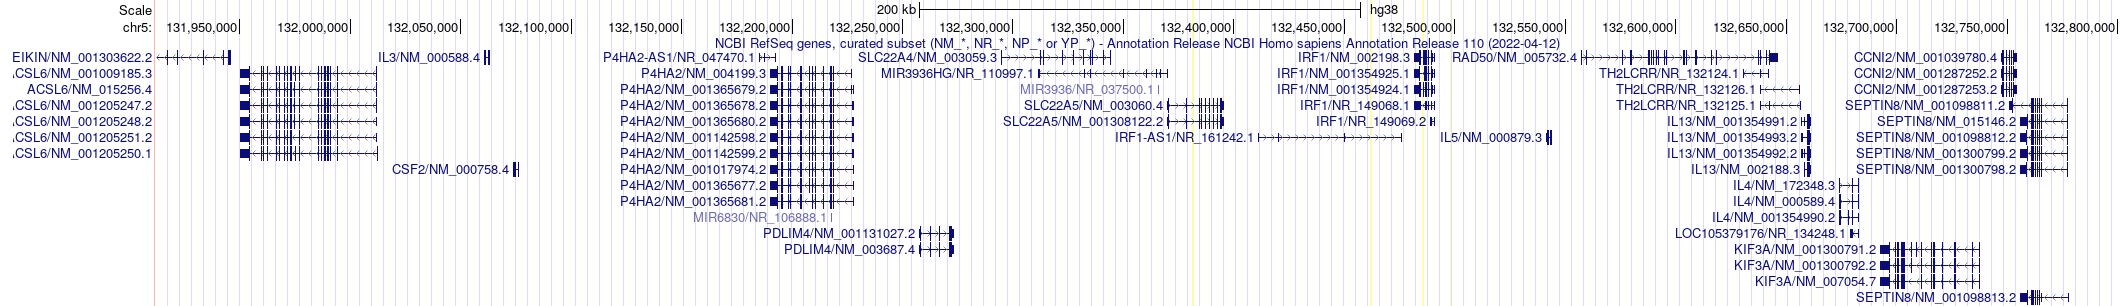
\includegraphics[width=\textwidth]{/home/gonzalez/Repositories/gwas2eqtl_pleiotropy/presentation_gold2022_paris/fig/chr5_131912097_132802472.png}
\end{center}

\small
\begin{itemize}
\item The cytokine locus: chr5:131,912,097-132,802,472. Genes IRF1, IL3, IL4, IL5, ...
\item Diseases: Allergy,Autoimmune dis.,Cancer of breast,Circulatory sys. dis.,Hypertension,Respiratory system dis.
\item For instance: rs2522051 regulates 12 e-genes in 23 e-tissues
\end{itemize}
\normalsize

\end{frame}

%%%%%%%%%%%%%%%%%%%%%%%%%%%%%%%%%%%%%%%%%%%%%%%%%%%%%%%%%%%%%%%%%%%%%%%%%%%%%%%%
\begin{frame}
\frametitle{Where are the pleiotropic variants?$^1$}

    \begin{center}
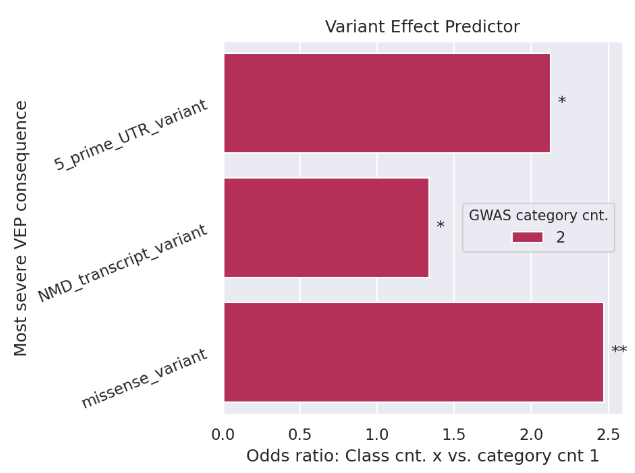
\includegraphics[width=0.7\textwidth]{/home/gonzalez/Repositories/gwas2eqtl_pleiotropy/out/gwas418/pval_5e-08/r2_0.1/kb_1000/window_1000000/pltbar_vep_consequence.py/vep.png}
     \end{center}

Upstream and downstream of genes and in the intron

\let\thefootnote\relax\footnotetext{$^1$https://www.ensembl.org/vep}
     
\end{frame}

%%%%%%%%%%%%%%%%%%%%%%%%%%%%%%%%%%%%%%%%%%%%%%%%%%%%%%%%%%%%%%%%%%%%%%%%%%%%%%%%
\begin{frame}
\frametitle{Do pleiotropic variants associate to more eQTL genes?}

\begin{columns}
\begin{column}{0.5\textwidth}
    \begin{center}
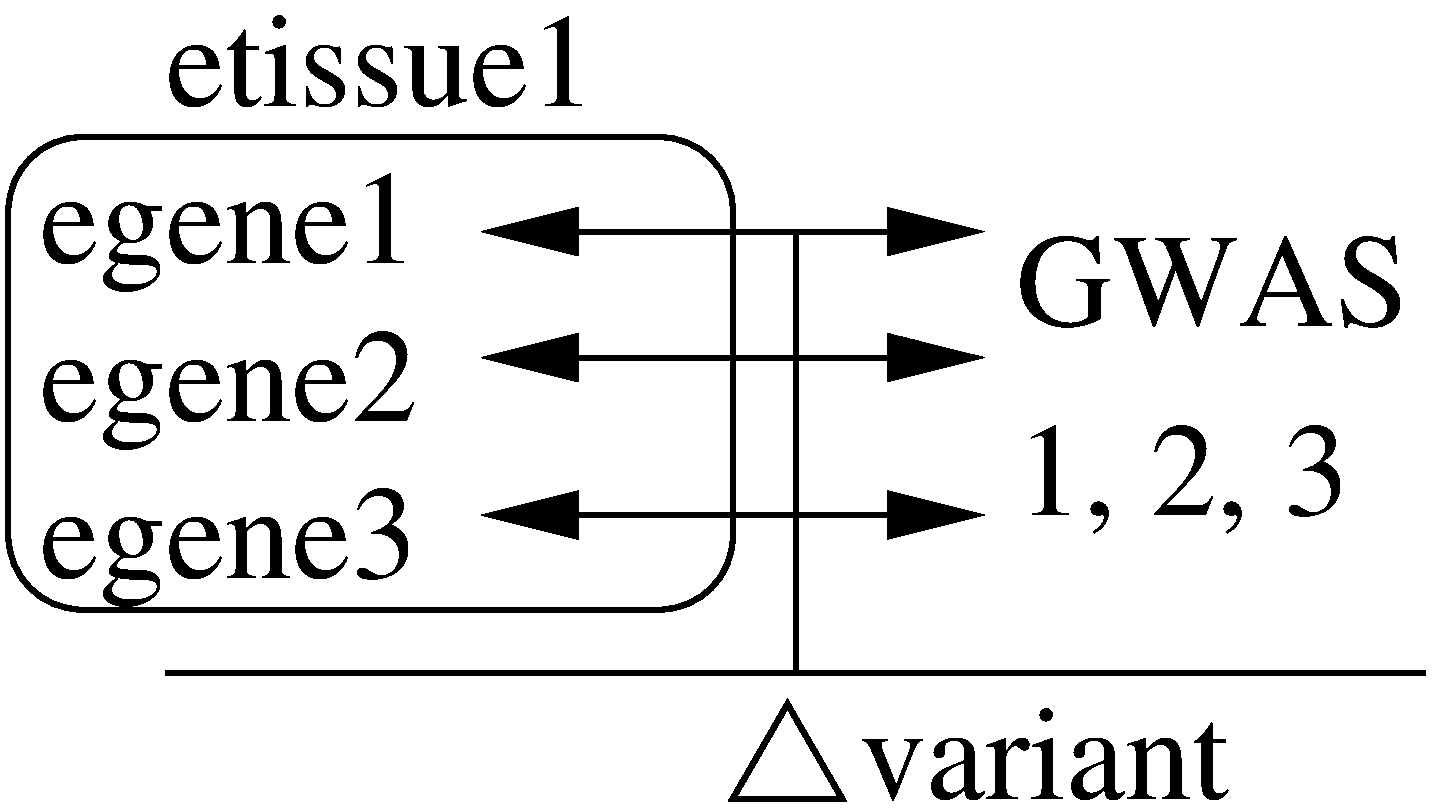
\includegraphics[width=0.7\textwidth]{/home/gonzalez/Repositories/gwas2eqtl_pleiotropy/presentation_gold2022_paris/fig/model_pleio_egenes.png}
     \end{center}
\end{column}
\begin{column}{0.5\textwidth}  %%<--- here
    \begin{center}
\includegraphics[width=\textwidth]{/home/gonzalez/Repositories/gwas2eqtl_pleiotropy/out/gwas418/pval_5e-08/r2_0.1/kb_1000/window_1000000/pltbar_x_per_variant_etissue_y_egene.py/plt.png}
     \end{center}
\end{column}
\end{columns}

\end{frame}

%%%%%%%%%%%%%%%%%%%%%%%%%%%%%%%%%%%%%%%%%%%%%%%%%%%%%%%%%%%%%%%%%%%%%%%%%%%%%%%%
\begin{frame}
\frametitle{Do pleiotropic variants associate to more eQTL tissues?}

\begin{columns}
\begin{column}{0.5\textwidth}
    \begin{center}
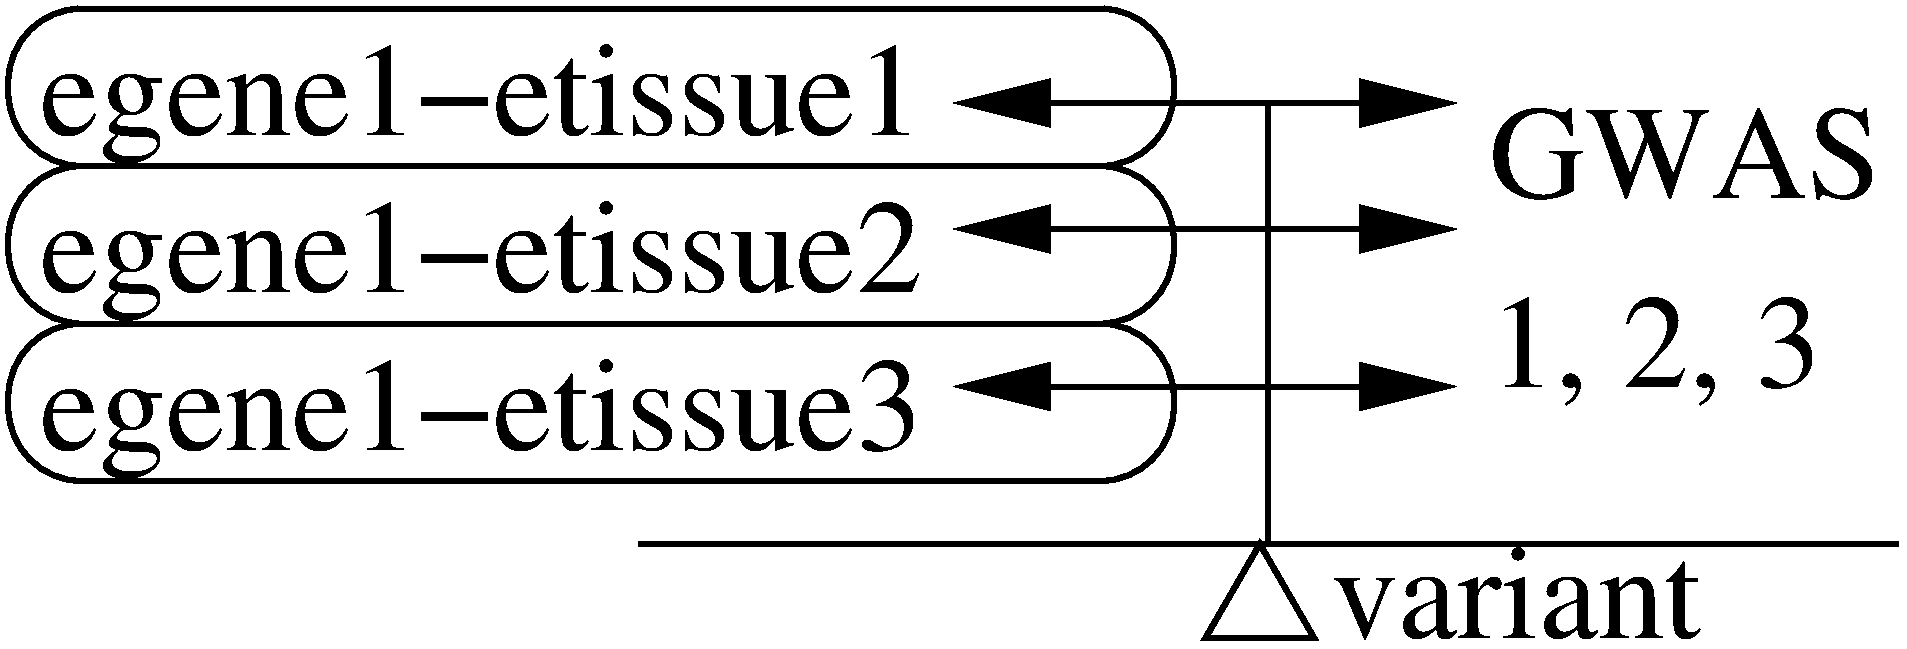
\includegraphics[width=0.7\textwidth]{/home/gonzalez/Repositories/gwas2eqtl_pleiotropy/presentation_gold2022_paris/fig/model_pleio_etissues.png}
     \end{center}
\end{column}
\begin{column}{0.5\textwidth}  %%<--- here
    \begin{center}
\includegraphics[width=\textwidth]{/home/gonzalez/Repositories/gwas2eqtl_pleiotropy/out/gwas418/pval_5e-08/r2_0.1/kb_1000/window_1000000/pltbar_x_per_variant_egene_y_etissue.py/plt.png}
     \end{center}
\end{column}
\end{columns}

\end{frame}

%%%%%%%%%%%%%%%%%%%%%%%%%%%%%%%%%%%%%%%%%%%%%%%%%%%%%%%%%%%%%%%%%%%%%%%%%%%%%%%%
\begin{frame}
\frametitle{Do pleiotropic variants bind more transcription factors?$^1$}

\begin{columns}
\begin{column}{0.5\textwidth}
    \begin{center}
\includegraphics[width=\textwidth]{/home/gonzalez/Repositories/gwas2eqtl_pleiotropy/out/gwas418/pval_5e-08/r2_0.1/kb_1000/window_1000000/pltbox_x_per_rsid_y_remapnr.py/bxplt_remaptf_per_rsid_flank_10.png}
     \end{center}
\end{column}
\begin{column}{0.5\textwidth}  %%<--- here
    \begin{center}
\includegraphics[width=\textwidth]{/home/gonzalez/Repositories/gwas2eqtl_pleiotropy/out/gwas418/pval_5e-08/r2_0.1/kb_1000/window_1000000/pltbar_x_per_variant_pleiotropy_y_remapcrm.py/remapcrm_flank10.png}
     \end{center}
\end{column}
\end{columns}

\let\thefootnote\relax\footnotetext{$^1$https://remap.univ-amu.fr}

\end{frame}

\section{Conclusions, perspective and acknowledgements} %%%%%%%%%%%%%%%%%%%%%%%%%%%%%%%%%%%%%%%%%%%%%%%%%%%%%%%%%%%%%%

%%%%%%%%%%%%%%%%%%%%%%%%%%%%%%%%%%%%%%%%%%%%%%%%%%%%%%%%%%%%%%%%%%%%%%%%%%%%%%%%
\begin{frame}
\frametitle{Concluding remarks}

Outcomes interesting for the GOLD population genotypes
%
\begin{itemize}
\item A large set of causal GWAS variants annotated with target genes and tissues
\item A list of pleiotropic variants and regions
\end{itemize}
%
\vfill
%
What are the gene regulatory properties underlying pleiotropy between complex traits?
%
\begin{itemize}
\item Variant pleiotropy is correlated in regions
\item Enrichment of variants upstream (incl. 5'UTR) and downstream of genes (incl. 3'UTR)
\item Enrichment of transcription factor and CRM binding
\item Increased number of associated egenes and etissues
\end{itemize}


\end{frame}

%%%%%%%%%%%%%%%%%%%%%%%%%%%%%%%%%%%%%%%%%%%%%%%%%%%%%%%%%%%%%%%%%%%%%%%%%%%%%%%%
\begin{frame}
\frametitle{Perspectives}


\begin{itemize}
\item A web portail to share data
\item Causality of eQTL genes on GWAS (Looking for experts ;-) )
\end{itemize}

\end{frame}

%%%%%%%%%%%%%%%%%%%%%%%%%%%%%%%%%%%%%%%%%%%%%%%%%%%%%%%%%%%%%%%%%%%%%%%%%%%%%%%%
\begin{frame}
\frametitle{Acknowledgements}

\begin{itemize}
\item L\'eopoldine Lecerf (M1)
\item P Paul, P Rihet, M Michel, S Marquet, S Spicuglia
\end{itemize}
%
\vfill
%
Funding
%
\begin{itemize}
\item Institut Cancer et Immunologie - Aix-Marseille Univ.
\item Agence nationale de la recherche (ANR)
\item GOLD
\end{itemize}

\end{frame}

%%%%%%%%%%%%%%%%%%%%%%%%%%%%%%%%%%%%%%%%%%%%%%%%%%%%%%%%%%%%%%%%%%%%%%%%%%%%%%%%
\begin{frame}
\frametitle{}

\end{frame}

%%%%%%%%%%%%%%%%%%%%%%%%%%%%%%%%%%%%%%%%%%%%%%%%%%%%%%%%%%%%%%%%%%%%%%%%%%%%%%%%
\begin{frame}
\frametitle{Do pleiotropic variants associate to more traits (after fixing egene-etissue)?}

\begin{columns}
\begin{column}{0.5\textwidth}
    \begin{center}
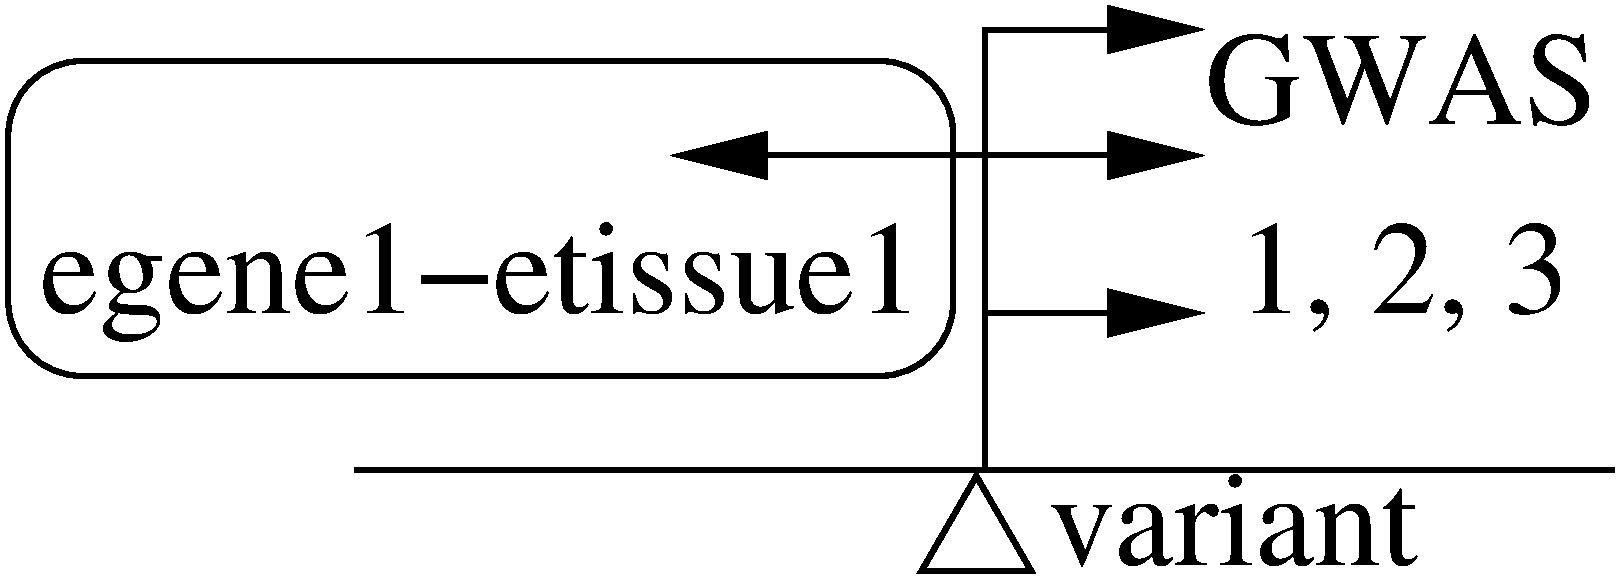
\includegraphics[width=0.7\textwidth]{/home/gonzalez/Repositories/gwas2eqtl_pleiotropy/presentation_gold2022_paris/fig/model_pleio_gwas.png}
     \end{center}
\end{column}
\begin{column}{0.5\textwidth}  %%<--- here
    \begin{center}
\includegraphics[width=\textwidth]{/home/gonzalez/Repositories/gwas2eqtl_pleiotropy/out/gwas418/pval_5e-08/r2_0.1/kb_1000/window_1000000/pltbar_x_per_variant_egene_etissue_y_gwas.py/plt.png}
     \end{center}
\end{column}
\end{columns}

\end{frame}

\end{document}


